\documentclass[tikz,border=2pt]{standalone}
\usepackage{amsmath,amssymb}
\usepackage{tikz}
\usetikzlibrary{matrix}

\begin{document}
% Leading principal submatrices A_1, A_2, A_3 nest in the top-left corner; Sylvester's
% criterion reads positive definiteness off the signs of their determinants.
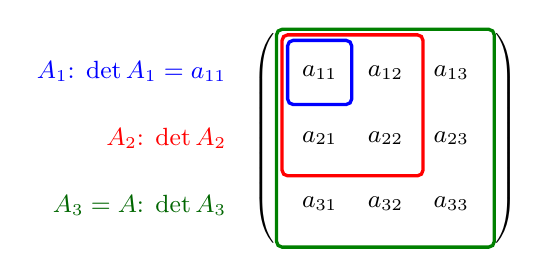
\begin{tikzpicture}[every node/.style={font=\small}]
	\matrix (A) [matrix of math nodes, nodes={minimum size=8mm, anchor=center}, left delimiter=(, right delimiter=), column sep=1pt, row sep=1pt] at (0,0) {
		a_{11} & a_{12} & a_{13} \\
		a_{21} & a_{22} & a_{23} \\
		a_{31} & a_{32} & a_{33} \\
	};
	\draw[blue, very thick, rounded corners=2pt] (A-1-1.north west) rectangle (A-1-1.south east);
	\draw[red, very thick, rounded corners=2pt] ([xshift=-2pt, yshift=2pt]A-1-1.north west) rectangle ([xshift=2pt, yshift=-2pt]A-2-2.south east);
	\draw[green!50!black, very thick, rounded corners=2pt] ([xshift=-4pt, yshift=4pt]A-1-1.north west) rectangle ([xshift=4pt, yshift=-4pt]A-3-3.south east);
	\node[blue, anchor=east] at (-1.9,0.85) {$A_1$: $\det A_1=a_{11}$};
	\node[red, anchor=east] at (-1.9,0.0) {$A_2$: $\det A_2$};
	\node[green!40!black, anchor=east] at (-1.9,-0.85) {$A_3=A$: $\det A_3$};
\end{tikzpicture}
\end{document}
